\section{Réécriture des numéros de Téléphone}

La réécriture de numéros téléphoniques s'adresse aux clients Privilège. Comme il l'a été dit dans la présentation de l'entreprise, ces clients détiennent un numéro Dynamease. Ce numéro permet aux appels entrant d'être redirigés sur un des appareils téléphoniques de l'utilisateur. Par contre il n'etait pas possible de passer un appel avec le numéro Dynamease.

Le but de cette fonctionnalité est de permettre à l'utilisateur Privilège, passant des appels depuis l'application téléphonique, d'avoir son numéro Dynamease affiché sur l'appareil téléphonique de la personne appelée.

\subsubsection{Étude du cahier des charges}

Le fonctionnement global de cette fonctionnalité est une redirection. L'utilisateur Privilège appelant un numéro, par l'application Dynamease, appellera en réalité un Trunk Dynamease. Un circuit est un circuit permettant le transport de plusieurs communication téléphonique. Une fois la communication créée sur le Trunk un appel est effectué depuis le numéro Dynamease vers la personne appelée par l'utilisateur.

Pour réaliser ce procédé on aura besoin du serveur téléphonique pour pouvoir rediriger les appels de l'utilisateur. Cette partie ne sera pas de mon ressort mais il sera effectué une explication de son fonctionnement. Cette explication est nécessaire à la compréhension du travail effectué par la suite.

Le serveur Dynamease jouera le rôle d'intermédiaire entre le serveur téléphonique et les applications téléphoniques. Des requêtes devront donc être crées pour gérer les communications nécessaire durant la procédure de réécriture de numéros.

Les applications téléphoniques auront pour rôle de vérifier les droits de l'utilisateur, et d'envoyer les requêtes vers le serveur avec les informations nécessaires pour faire fonctionner ce procédé.

\subsubsection{Fonctionnement du serveur téléphonique}

Le serveur téléphonique aura pour rôle de lier deux communications. Lors de l'appel de l'utilisation de la réécriture par l'utilisateur, celui-ci est redirigé vers un numéro de Trunk. Une fois la communication établie avec le Trunk, une nouvelle communication est établie. Un appel, depuis le numéro Dynamease de l'utilisateur vers l'appelant, est émis. Une fois cette appel effectué, les deux communications, sont alors liées. Ainsi l'utilisateur est en communication avec son correspondant, en passant par son numéro Dynamease.

Lors d'un appel entrant vers le Trunk, une requête doit être envoyée vers le serveur Dynamease afin de déterminer si le numéro entrant appartient à un client Privilège et également pour récupérer le numéro Dynamease de ce client.

Le serveur Téléphonique doit donc récupérer les informations suivantes :

\begin{itemize}
	\item Les numéros de téléphone de l'utilisateur Privilège;
	\item Le numéro de téléphone de redirection.
\end{itemize}
 

\subsubsection{Le serveur Dynamease}

Le serveur Dynamease aura pour rôle de communiquer les informations entre les applications téléphoniques et le serveur téléphonique. Plusieurs requêtes doivent donc être créées. La communication entre les différents services est représentée par le diagramme suivant :\\

\begin{figure}[!h]
	\centering
	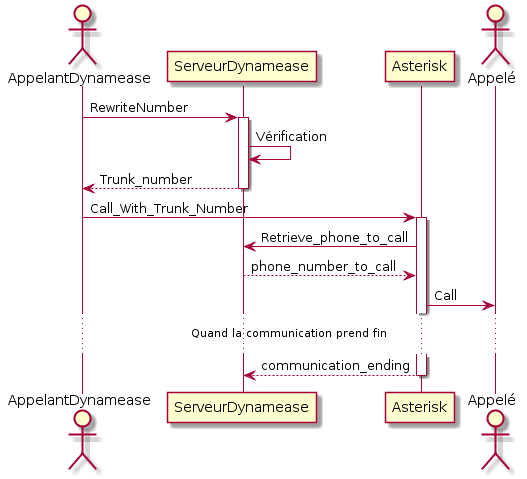
\includegraphics[scale=0.8]{img/sequence_rewirte.png}
	\caption{\label{sequence_rewirte} Diagramme de séquence de la ré-écriture de numéro}
\end{figure}

Nous voyons sur ce diagramme que le procédé est initié par les applications téléphoniques, nous allons donc commencer par la présentation du fonctionnement des requêtes utilisées par les applications téléphoniques.
\newpage

\begin{figure}[!h]
	\centering
	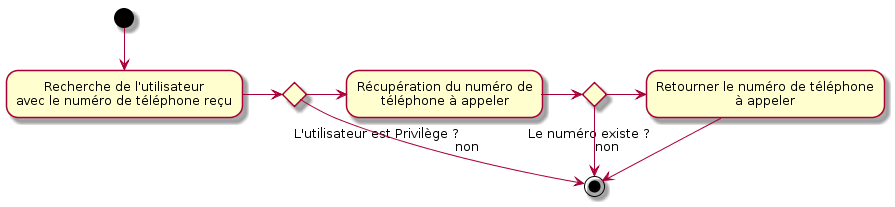
\includegraphics[scale=0.5]{img/activity_rewrite_ast.png}
	\caption{\label{activity_rewrite_ast} Diagramme d'activité de la méthode appelée par le serveur Asterisk}
\end{figure}


L'application téléphonique devra envoyée une requête au serveur pour indiquer que l'utilisateur souhaite effectuer une réécriture de numéro. Cette requête devra contenir le numéro à appeler ainsi que l'Id de l'utilisateur voulant passer l'appel. Une réponse est alors renvoyé avec le numéro de téléphone à joindre. L'application téléphonique aura alors pour rôle de lancer un appel vers ce numéro de téléphone. 

Plusieurs choix sont possible en ce qui concerne la réponse renvoyée lorsque la requête est envoyé de la part d'un utilisateur non privilège. Soit nous renvoyons une requête indiquant à l'utilisateur qu'il ne détient pas des droits nécessaires pour effectuer ce genre d'appel. Soit nous renvoyons le numéros de téléphone passé en paramètre de la requête. C'est cette dernière qui est choisie, car elle permet quand même à l'appel d'être effectué.

Le numéro à appeler sera stocké en mémoire du serveur dans un objet de type dictionnaire, ayant pour clef l'identifiant du client privilège et pour valeur le numéro à appeler. Ainsi nous permettons aux utilisateurs de pouvoir passer par l'historique d'appel de leur téléphone pour contacter le dernier contact appelé depuis leur numéro Dynamease.\\

On a noté dans la partie précédente les différentes informations que devaient détenir le serveur téléphonique. Les différents numéros d'un utilisateurs Dynamease sont stockés sur le serveur. Il est donc aisé de récupérer ces informations, afin de déterminer si un numéro entrant appartient à l'utilisateur. De plus les numéros de Trunk peuvent être considérés comme des constantes. Il est donc préférable que celles-ci soient stockées dans les fichiers de configuration du serveur Dynamease. En revanche cette technique ne marchera que pour le dernier contact appelé grâce à la réécriture de numéro. Pour rappeler des anciens contacts il faudra, soit passer par l'historique d'appel de Dynamease, la liste de contact ou l'option numérotation de Dynamease.
\newpage
\begin{figure}[!h]
	\centering
	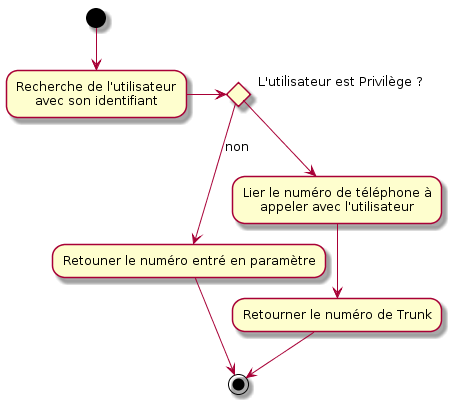
\includegraphics[scale=0.7]{img/activity_rewrite_app.png}
	\caption{\label{activity_rewrite_app} Diagramme d'activité de la méthode appelée par les applications téléphoniques}
\end{figure}

La meilleur solution est de créer une requête permettant au serveur téléphonique de vérifier si un numéro correspond à un utilisateur donné et si il détient les droits privilèges. La réponse renvoyée correspondra au numéro que l'utilisateur Privilège souhaite joindre. Si l'appel ne provient pas d'un utilisateur Privilège, la réponse indiquera au serveur téléphonique de mettre fin à l'appel. Cette requête sera effectuée à chaque appel entrant sur le Trunk présent sur le serveur téléphonique.

\subsubsection{Les applications téléphoniques}

Les applications téléphoniques doivent envoyer une requête vers le serveur Dynamease dès que l'utilisateur sélectionne l'appel d'un contact. L'application doit également fournir le numéro à appeler.

Avant tout envoie de requête, une vérification sur le type de contact de l'utilisateur est effectuée. Que ce soit pour Iphone ou pour Android, le stockage des informations de l'utilisateur est géré de la même manière. Un procédé de type clef valeur (dictionnaire) persistant est présent sur les deux applications. Ce dictionnaire est rempli lors de la connexion de l'utilisateur. Il nous suffit donc ici de vérifier si l'utilisateur détient bien les droits avant d'envoyé cette requête. Bien que le serveur effectue également cette vérification, il est important d'effectuer cette vérification en amont pour ne pas surcharger le serveur de requêtes inutiles.\\

Dans les deux applications, les contacts sont rangés en deux catégories, les contacts Dynamease et les contacts du téléphone. Les contacts du téléphone sont pourvus d'un numéro de téléphone alors que les contacts Dynamease n'ont que leur identifiant Dynamease. Donc selon le contact à appeler, l'application doit soit envoyer un numéro de téléphone ou le numéro de l'identifiant Dynamease du contact.

\section{Le Click2Call}

Le Click2Call sera proposé comme une option, limitée dans le temps, pour tous les clients Dynamease. Cette option permettra aux clients de disposer de cartes de visite virtuelles publiques, qu'ils pourront déposer sur des sites internets. Ces cartes de visite permettront aux clients d'être contactés grâce à elle en un seul clique. Cet appel se fera sans échange de numéro de téléphone. C'est à dire que l'appelant ne verra pas le numéro du client et inversement.

\subsubsection{Étude du cahier des charges}

Pour réaliser cette fonctionnalité nous avons besoin de mettre en relation deux personnes sans échange de numéro. Le serveur téléphonique sera utilisé afin de créer un lien entre les deux communicant. Je ne serais, encore une fois, pas en charge de cette partie du développement mais nous aborderons le fonctionnement global de cette partie.

Nous allons avoir besoin du serveur Dynamease qui sera en charge d'orchestrer les échanges d'informations avec le serveur téléphonique et les applications téléphoniques.

Les applications téléphoniques devront également être changées dans le but de pouvoir recevoir les informations des appels.

\subsubsection{Fonctionnement du serveur téléphonique}

Le serveur téléphonique aura pour charge, la liaison entre les deux interlocuteurs grâce à des conférences. Ces conférences ne seront accessible que par l'appelant et l'appelé, une requête est donc crée pour récupéré les conférence liées aux numéros de téléphone renseignés. Les conférences sont désignées par un identifiant unique, leur nom.

Pour accéder à une conférence, il faut faire intervenir un numéro de Trunk. C'est ce numéro qui sera affiché sur les appareils téléphoniques des deux interlocuteurs, car leur appel se fera vers le numéro de Trunk. Ainsi aucun des deux interlocuteurs n'aura le numéro de téléphone de l'autre interlocuteur.

\subsubsection{Le serveur Dynamease}

Le serveur Dynamease aura pour rôle la gestion du fonctionnement du Click2Call. Nous avons vu précédemment qu'il faut créer des conférences pour chacun des appels. Ces conférences devront donc être créées et stockées jusqu'à leur destruction. Un cycle de vie nous servira donc pour gérer toutes ces conférences et éviter une surcharge du serveur.

Les conférences passent par plusieurs étapes. La première étape est la création, à ce moment la conférence est ajouté à la liste des conférences et est identifié par un nom unique (ce nom est généré aléatoirement). Par la suite, la conférence passe en attente, c'est à dire que cette conférence est à disposition pour être utilisée par le serveur téléphonique. Lors de l'utilisation de cette conférence, son statut passe en mode attribuée, dans ce cas là elle ne peut plus être attribuée, jusqu'à ce que cette conférence soit terminée. Une fois terminée, la conférence repasse en attente. Ainsi on peut réutilisé plusieurs fois la même conférence est ainsi réduire le nombre d'objet conférence à stocker en mémoire.

Avant l'attribution de conférence on vérifie que le client Dynamease appelé n'est pas déjà présent dans une autre conférence. Ainsi on peut avoir une meilleure gestion des conférences, et identifier la disponibilité de l'utilisateur.

La liste de conférence, peut être accédée à tout moment, il faut donc gérer les problèmes de concurrence sur cette liste. On utilise donc la synchronisation des méthodes fournie par Java. Ces méthodes permettent de gérer l'accès à une liste par plusieurs Threads. Cette méthode gère une liste FIFO (First In First Out) de Thread, la liste n'est accessible que par un seul Thread à la fois, ce qui permet d'éviter les problèmes de concurrence.\\

L'accès à la conférence peut se faire de deux manière, soit par un appel vers le numéro du Trunk, soit un appel est émis de la conférence vers un utilisateur. La personne appelante utilisant le Click2Call sera forcément amenée vers la conférence, par un appel vers celle-ci. En ce qui concerne l'utilisateur Dynamease, il faut décider de la manière dont il sera amené vers la conférence. 

En passant l'appel depuis la conférence, l'application Dynamease n'aura qu'à afficher les informations clients, comme elle le fait habituellement. En utilisant la seconde solution, l'application Dynamease devra effectuer un appel vers la conférence, mais les charges d'appel pour Dynamease seront diminuées. Pour des raisons économiques, c'est ce second choix qui sera utilisé. De plus avec cette seconde solution, le prix de cette option pourra s'effectuer grâce à des appels surtaxés.\\

La procédure utilisé par cette fonction est la suivante :

\begin{figure}[!h]
	\centering
	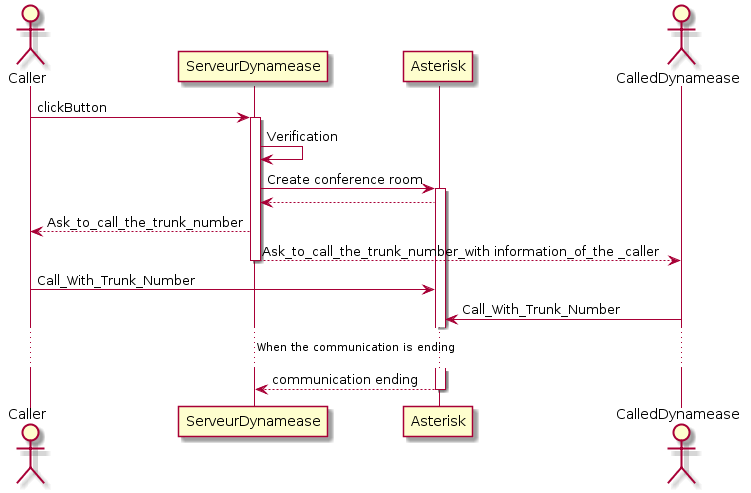
\includegraphics[scale=0.7]{img/sequence_click2call.png}
	\caption{\label{sequence_click2call} Diagramme de séquence de la fonctionnalité du Click2Call}
\end{figure}

Une personne appuie sur le bouton Click2Call. Ce bouton envoie une requête au serveur Dynamease contenant l'identifiant de l'utilisateur Dynamease à appeler ainsi que le contexte dans lequel s'effectue l'appel (type de site, objet vendu ...). A la réception de la requête, le serveur Dynamease vérifie qu'il existe des conférences disponible, s'il n'en existe pas le serveur en créée une nouvelle et de mande sa création au serveur téléphonique. Ensuite le serveur vérifie si l'utilisateur à joindre est disponible. Si cette vérification s'est effectuée sans problème, l'objet conférence est modifié avec les informations sur les numéros de téléphone pouvant y accéder. Le numéro du Trunk est envoyé à l'appelant. Ensuite une notification de type Click2Call est envoyé à l'utilisateur Dynamease avec le numéro de la conférence et les informations de cet appel.

La conférence démarre dès que les deux protagonistes entrent dans la conférence. Elle se termine quand un des deux protagoniste coupe la communication. A la fin de cette conférence une requête est envoyée au serveur Dynamease pour l'informer que la conférence peut être réattribuée.\\

En plus de ces requêtes, d'autres requêtes, spécifique à Dynamease, ont été créées dans l'objectif de gérer les différents numéros de conférence. Ajouter des numéros de conférence, et lister les informations pouvant être récupéré  sur les numéros de conférence.

\subsubsection{Les application téléphonique} 

Les applications téléphoniques doivent, à l'arrivée d'une notification Click2Call, générer un appel vers le numéro de Trunk, dans le but d'accéder à la conférence.

Dans cette notification il doit être présent les informations sur l'appelant. Pour cela on utilise le même principe déjà existant sur les notifications d'appel.\\

La gestion des notifications étant différentes selon le système d'exploitation il est important de bien différencier les deux types de notification. Nous allons commencer par les applications Android.

Les notifications d'appel, sont affichées par le biais du système Toast. Un toast est une fenêtre s'affichant obligatoirement au premier plan. La fenêtre Toast est donc affichée au premier plan même lors d'un appel, ce qui permet aux utilisateurs de lire les informations même si la fenêtre d'appel est affichée. Cette fenêtre est affichée pendant une courte durée, mais il est possible de laisser cette fenêtre affichée plus longtemps en utilisant le principe de \textit{timer} pour demander l'affichage du Toast à intervalle de temps réguliers. Les informations sont donc affichées pendant un laps de temps suffisamment long pour que l'utilisateur puisse lire toutes les informations récupérées sur l'appelant.

Lors de la réception de cette notification, l'utilisateur doit décider s'il veut répondre à l'appel. Ce qui signifie que la notification doit permettre la gestion d'actions de la part de l'utilisateur. Android ne permet la gestion des actions avec les Toasts. Cette notification doit simuler un appel. Un appel sur Android est représenté par une vue en plein écran. On peut reprendre ce principe en créant une activité. Cette activité affichera les informations de l'appelant, ainsi que deux boutons pour laisser le choix à l'utilisateur d'accepter ou de refuser l'appel.

Il est également possible de récupérer certaines informations de l'utilisateur comme la sonnerie utilisée par défaut des appel. On peut donc faire retentir cette sonnerie afin que l'utilisateur ai la sensation d'un appel. La fenêtre suivante est affiché sur le portable

[mettre Image]

En appuyant sur le bouton répondre, la fenêtre se ferme, et un appel est émis vers le numéro de conférence. Ainsi l'expérience utilisateur n'est pas altéré, car la sensation d'appel reste la même.\\

En ce qui concerne l'application Iphone, il est impossible d'avoir la même expérience utilisateur que pour la partie Android. Il n'est pas possible d'afficher des notifications spéciales si l'application n'est pas au premier plan. La notification Click2Call  doit donc être affichée comme une notification Iphone normale. Comme pour l'application Android, il faut laisser le choix à l'utilisateur de répondre où non à l'appel. Pour cela une fonctionnalité récente de IOS, disponible depuis la version 8, permet d'ajouter des boutons d'actions aux notifications. En ce qui concerne la notification sonore, il est possible d'avoir le même principe que les applications Android.


\section{L'appel depuis l'historique}

\begin{figure}[!h]
	\centering
	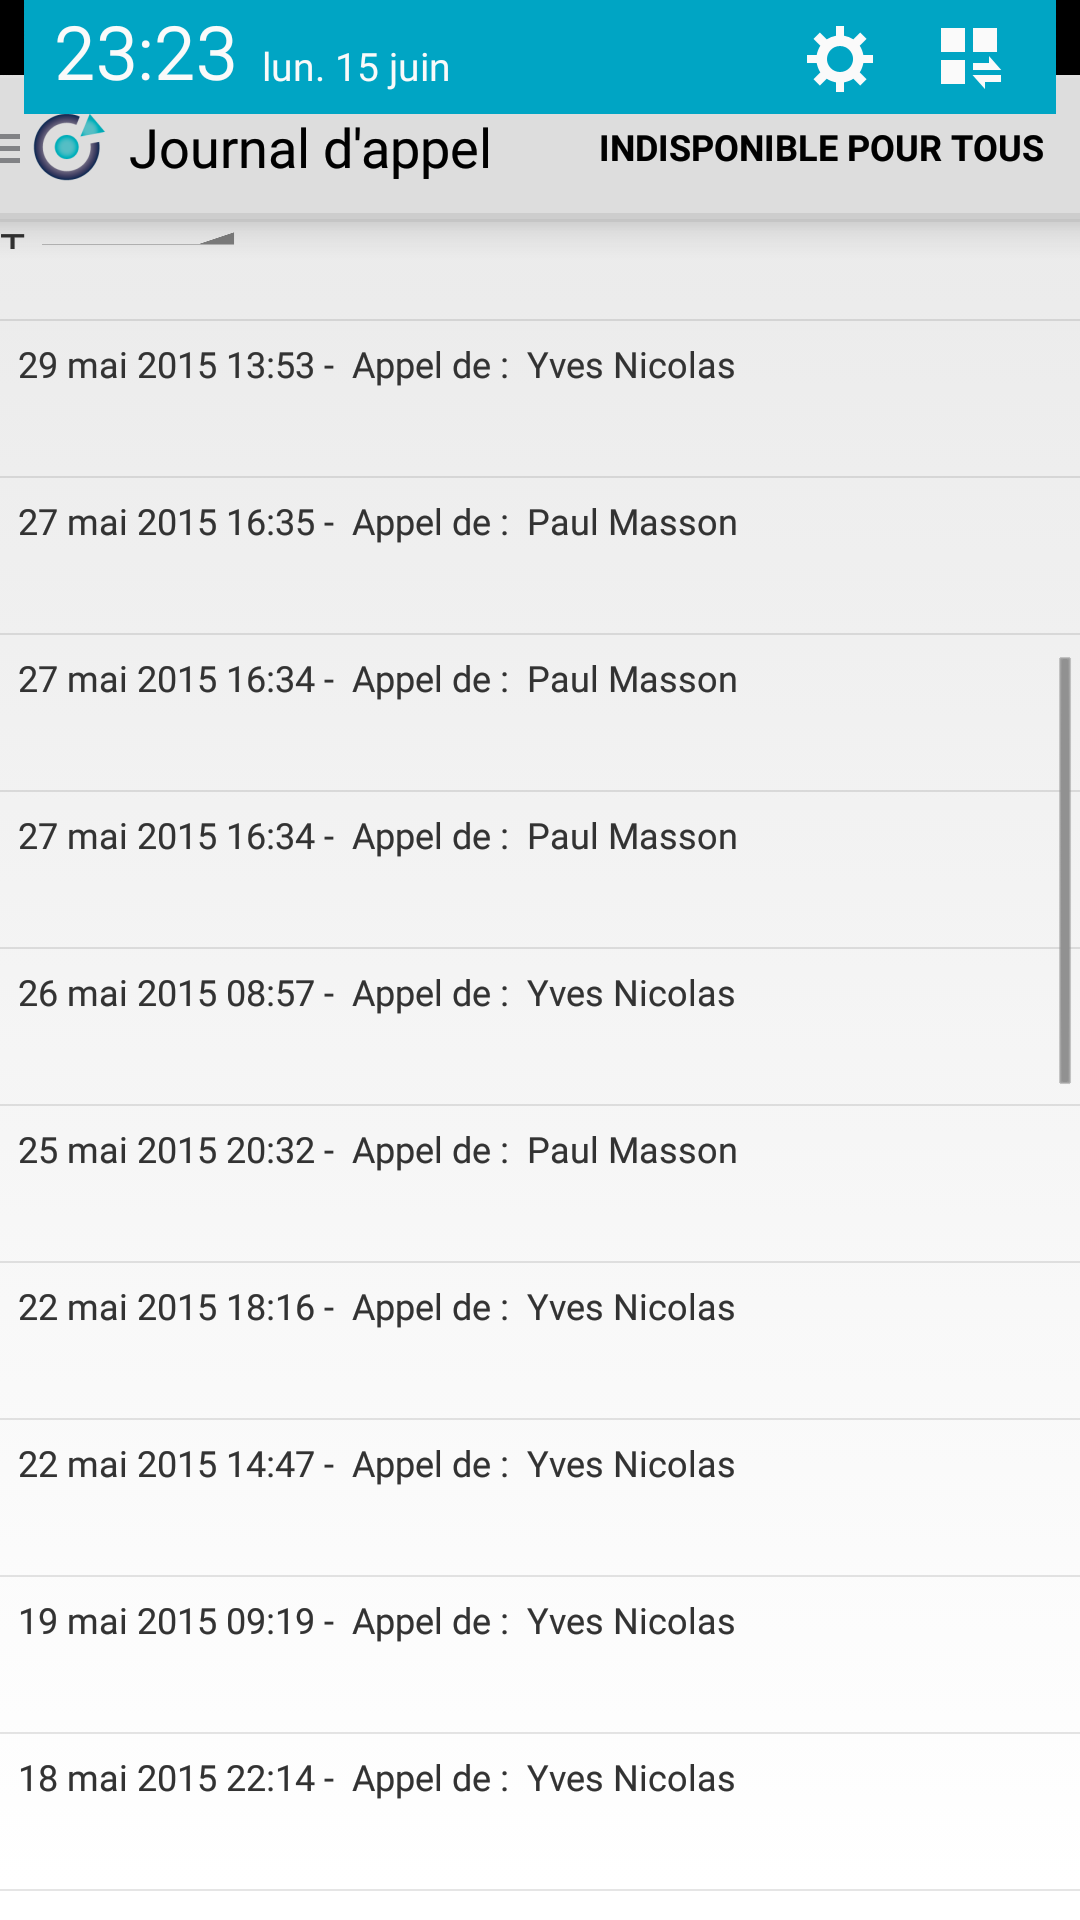
\includegraphics[scale=0.1]{img/historique.png}
	\caption{\label{historique} {Vue de l'historique d'appel sur l'application Android}}
\end{figure}

Les applications téléphoniques disposent d'un historique d'appel. Celui-ci nous indique la date et l'heure d'un appel, ainsi que d'éventuels informations sur l'appelant. Par contre il n'est pas possible de rappeler les contacts depuis cet historiques. Il est donc question de pouvoir effectuer ce rappel.

\subsubsection{Étude du cahier des charges}

Pour réaliser cette fonctionnalité nous avons besoin de faire une modification sur la base de données MySQL. En effet, la table représentant les appels ne stocke pas les informations nécessaire au rappel du contact, comme le numéro de téléphone ou l'identifiant Dynamease. Il faut donc rajouter ces informations dans la base de données. Cette modification sera effectuée par une autre personne. Quant à moi je serais en charge des modifications à effectuer sur les applications téléphoniques.

Je dois faire les modifications nécessaire pour que les applications téléphoniques gèrent cette nouvelle fonctionnalité.

\subsubsection{Les modifications}

La récupération des informations nécessaires se font via un objet Json. Le traitement de cet objet est différents selon le système d'exploitation téléphonique.

Pour les applications Android, le traitement se fait via un Mapper. Le Mappe est chargé de traduire une chaîne de caractère formé comme un objet Json en un autre objet passé en paramètre. L'objet Json, pour rappel se présente comme un dictionnaire (clefs, valeurs). Les clef représente les noms de variable et les valeurs, les valeurs prisent par les variables.

En ce qui concerne les applications Iphone, le procédé est manuel. L'objet voulue doit être récréé, contrairement à Android, où l'objet utilisé est le même que celui utilisé sur le serveur Dynamease. 

Maintenant que ces informations sont récupérées, il suffit simplement d'effectuer les mêmes tâches que pour un appel depuis la liste de contact.

\subsubsection{Amélioration de la base de données}

Après cette mise en place j'ai observé les modifications de la base de données. J'ai remarqué quelques erreurs effectuée sur celle-ci.

\newpage
\begin{figure}[!h]
	\centering
	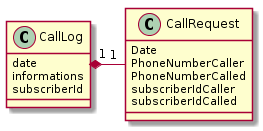
\includegraphics[scale=1]{img/classeCallLogOld.png}
	\caption{\label{class_callLog_old} Diagramme de classe de la table représentant l'historique d'appel}
\end{figure}

On vois que cette base de données ne respecte pas le terme de clef unique en effet. Il est possible que la valeur de date soit identique pour deux entrées.

La cardinalité entre ces deux tables, signifie que les informations présentent sur $"call_request"$ pourraient être présente sur la table $"call_log"$

Je pense donc que la partie de la base de données représentant l'historique d'appel pourrai être remplacé par la table suivante :

\begin{figure}[!h]
	\centering
	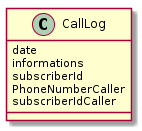
\includegraphics[scale=1]{img/classeCallLogNew.png}
	\caption{\label{class_callLog_new} Proposition d'amélioration du diagramme de classe de la table représentant l'historique d'appel}
\end{figure}

La première solution fût prise pour éviter les modifications sur une table déjà existante et risquer de perdre des données clients. 